\documentclass{article}
\usepackage[cm]{fullpage}
\usepackage{tikz}
\usepackage{graphicx}
\usepackage{hyperref}
\usepackage{natbib}
\usepackage{amsmath,amssymb}
\DeclareMathOperator*{\argmin}{arg\,min}
\DeclareMathOperator*{\Diag}{Diag}
\DeclareMathOperator*{\TPR}{TPR}
\DeclareMathOperator*{\FPR}{FPR}
\DeclareMathOperator*{\argmax}{arg\,max}
\DeclareMathOperator*{\maximize}{maximize}
\DeclareMathOperator*{\minimize}{minimize}
\newcommand{\RR}{\mathbb R}

\begin{document}

\title{Benchmarking fpop}
\author{RM, TDH, PF, GR}
\maketitle

\tableofcontents

\section{Empirical evaluation of fpop}

As explained in section \ref{sec:simil-diff-betw} functional pruning
leads to a better pruning in the following sense: any point pruned by
inequality-based pruning will also be pruned by functional pruning.
However, functionnal pruning is computationnaly more demanding than
inequality based pruning.  We thus decided to empirically compared the
performance of FPOP to PELT, pDPA and binary segmentation (binseg).

To do so, we implemented FPOP for the quadratic loss in C++.
More precisely, we considered the cost $C(y_{\tau_j+1:\tau_{j+1}} = \sum_{t=\tau_j+1}^{\tau_{j+1}} (y_t - \bar{y}_{\tau_j+1:\tau_{j+1}})^2,$ where
$ \bar{y}_{\tau_j+1:\tau_{j+1}} = \frac{1}{\tau_{j+1} - \tau_j} \sum_{t=\tau_j+1}^{\tau_{j+1}} y_t$.
We assessed the runtimes of FPOP on both real microarray data as well as synthetic data.

There are several differences between FPOP and the other
algorithms, as shown in the table below.
\begin{center}
  \begin{tabular}{ccccc}
    algorithm & models computed & optimal? & implementation & runtime as a function of segments $K$\\
    \hline
    FPOP & 1 & yes & C++  &  ?                  \\
    PELT & 1 & yes & C++  &  decrease \\
    pDPA & $K_{max}$ & yes & C++ & increase \\
    Binseg & $K_{max}$ & no & C++ & increase
  \end{tabular}
\end{center}

Note that the Binary segmentation heuristic is computationally
extremely fast. That is because its complexity is on average in
$\mathcal{O}(n \log K_{\text{max}})$. Furthermore, it relies on a few
fairly simple operations and hence the constant in front of this big
$\mathcal O$ notation is expected to be quite low.  For this reason we
believe that binary segmentation is good reference point in terms of
speed and we do not think it is possible to be much faster.


\subsection{Speed benchmark: 4467 chromosomes from 
  tumor microarrays}

\citet{HOCKING-SegAnnDB} proposed to benchmark the speed of 
segmentation algorithms on a database of 4467 problems of size varying
from 25 to 153662 data points. These data come from different
microarrays data sets (Affymetrix, Nimblegen, BAC/PAC) and different
tumor types (leukemia, lymphoma, neuroblastoma, medulloblastoma).

We compared fpop to several other segmentation algorithms: pDPA
\citep{pruned-dp}, pelt \citep{pelt}, and binary segmentation
(binseg).  For such data, we expect a small number of changes and for
all profiles we ran pDPA and binseg with a maximum number of changes
$K_{\text{max}}=52$.  In this scenario we expect binary segmentation
to be particularly efficient as its complexity is on average in
$\mathcal{O}(n\log K_{max})$.

We used the R \verb|system.time| function to measure
the execution time of all 4 algorithms on all 4467 segmentation
problems. The R source code for these timings is in
\verb|benchmark/systemtime.arrays.R| in the opfp project repository on
R-Forge:
\url{https://r-forge.r-project.org/projects/opfp/}


It can be seen in Figure~\ref{fig:sys_runtimes_microarray} that in
general fpop is faster than pelt and pDPA, but about two times slower
than binseg.  Note that \verb|system.time| is inaccurate for small
times, as pointed out in Figure~\ref{fig:sys_runtimes_microarray}
middle and right.  For these small profiles we also assessed the
performances of fpop, pelt and binseg using the \verb|microbenchmark|
package and confirmed that fpop is faster than pelt. For these small
problems we were surprised to observe that fpop exhibited about the
same speed as binseg (microbenchmark results figure not shown).
 
\begin{figure}\label{fig:sys_runtimes_microarray}
 \parbox{7.5cm}{ 
   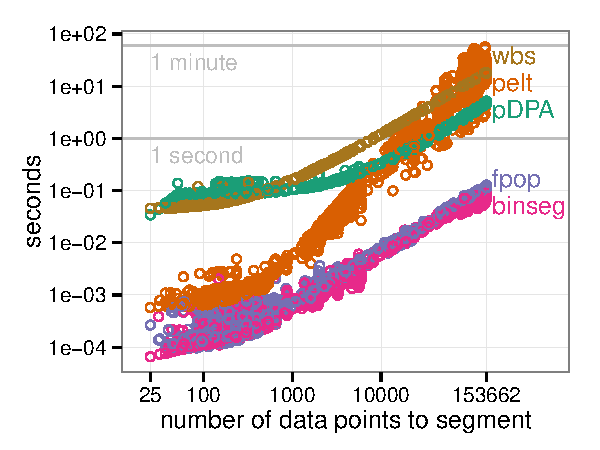
\includegraphics[width=\linewidth]{figure-systemtime-arrays-small}
  }
  \parbox{11.5cm}{  
    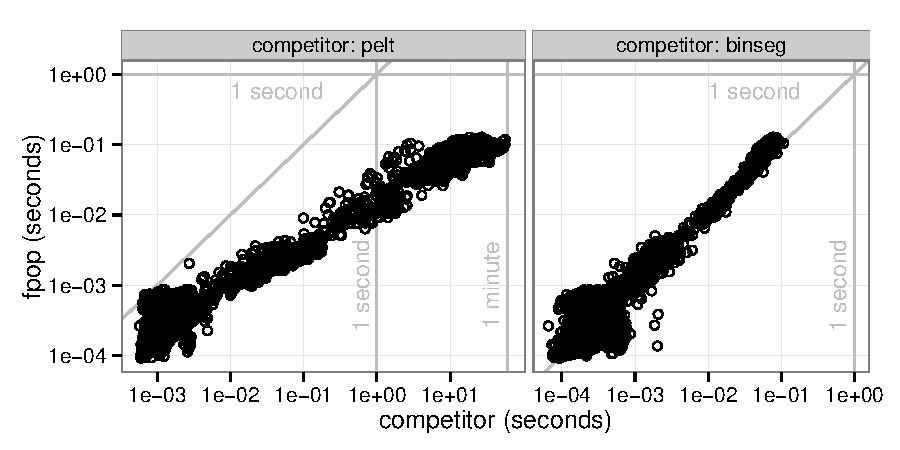
\includegraphics[width=\linewidth]{figure-systemtime-arrays-fpop-pelt-small}
  }
  %\parbox{6cm}{ 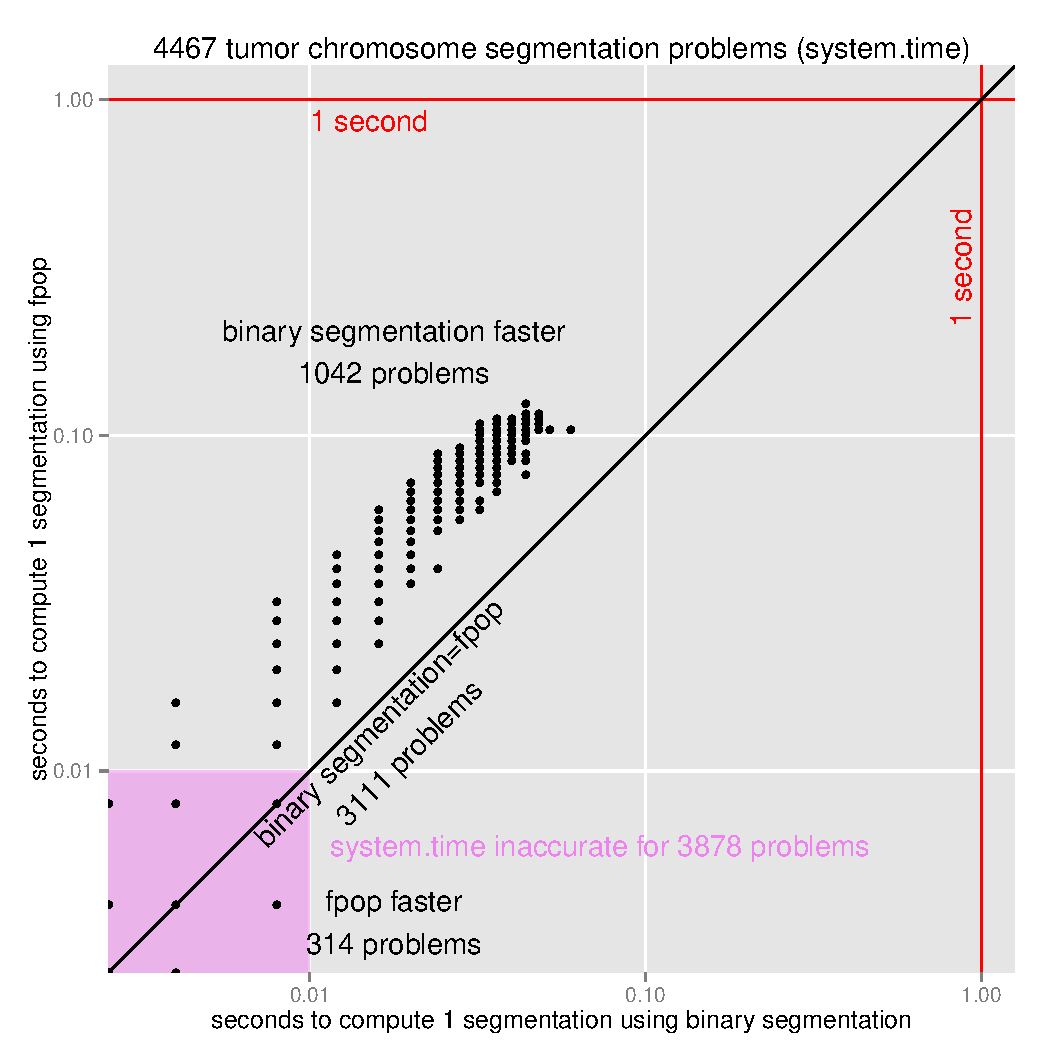
\includegraphics[height=5cm]{figure-systemtime-arrays-fpop-multiBinSeg}}
  \caption{Left) Runtimes of fpop, pelt, pDPA and Binseg as a function
    of the length of the profile using on the neuroblastoma tumor micro array
    benchmark.  Middle) Runtimes of pelt and fpop for the same
    profiles.  Right) Runtimes of Binseg and fpop for the same
    profiles.  }
\end{figure}





\subsection{Speed benchmark: simulated data with different 
  number of changes}

The speed of Pelt, Binseg and pDPA depends on the underlying number of changes.
For pDPA and Binseg the relationship is clear as to cope with a larger number of changes
one need to increase the maximum number of changes to look for $K_{max}$. 
For a fixed size signal the runtime depency is expected to be in $\log(K)$ for Binseg and
in $K$ for pDPA.

For PELT the relationnship is less clear, however we expect pruning to be more efficient
if there is a large number of change-points. Hence for a fixed size signal we expect 
the runtime of Pelt to improve with the underlying number of change.

Based on section \ref{sec:simil-diff-betw} we expect fpop to be more efficient than pelt and pDPA.
Thus it seems reasonable to expect fpop to be efficient for the whole range of $K$. 
This is what we empirically checked in this section.

To do that we simulated Gaussian signal with 200000 data points and varied the number of changes
and timed the algorithms for each of these signals. We then repeat the same experience for signals with $10^7$ and timed fpop and Binseg only.
The R source code
for these timings is in \verb|benchmark/systemtime.simulation.R| in
the opfp project repository on R-Forge: \url{https://r-forge.r-project.org/projects/opfp/}.

It can be seen on figure \ref{fig:simu_numberK} that fpop is always faster than pDPA and pelt. 
Interestingly for both $n=2\times 10^5$ and $10^7$ it is faster than binseg for a true number of change-point larger than 500.


\begin{figure}\label{fig:simu_numberK}
  \begin{center}
    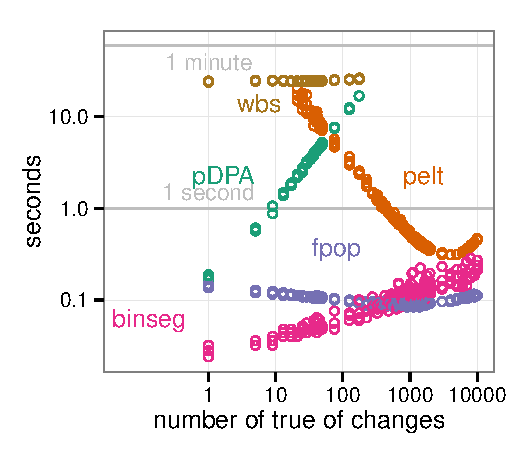
\includegraphics[width=8cm]{figure-systemtime-simulation-small}
    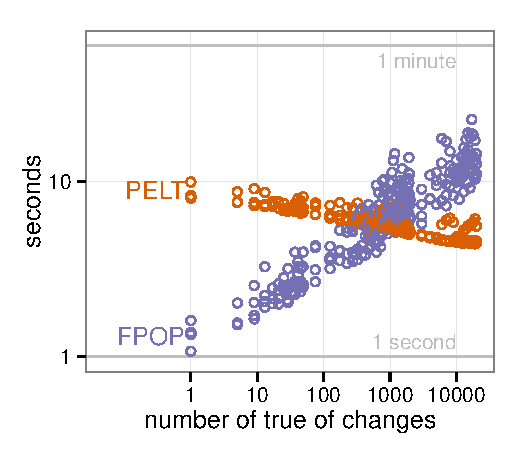
\includegraphics[width=8cm]{figure-systemtime-simulationLarge-small}
  \end{center}
\caption{Runtimes as a function of the true number of change-points.
Left) For fpop, pelt,
pDPA and Binseg and $n=2. 10^5$
Right) For Binseg and fpop and $n=10^7$
}
\end{figure}



\subsection{Accuracy benchmark: the neuroblastoma data set}

\begin{table}
  \centering
  \parbox{3in}{
    % latex table generated in R 3.2.2 by xtable 1.7-4 package
% Mon Sep 21 13:35:40 2015
\begin{tabular}{rrr}
  \hline
 & mean & sd \\ 
  \hline
WBS & 3.87 & 1.69 \\ 
  WBS.default & 72.67 & 6.49 \\ 
  SMUCE.default & 70.95 & 7.41 \\ 
  SMUCE & 2.43 & 1.00 \\ 
  PELT.default & 8.01 & 4.91 \\ 
  FPOP & 2.20 & 1.01 \\ 
  pDPA & 2.20 & 1.01 \\ 
  PELT & 2.20 & 1.01 \\ 
  BinSeg & 2.20 & 0.93 \\ 
   \hline
\end{tabular}

  }
  \parbox{3in}{
    % Created by tikzDevice version 0.7.0 on 2015-09-03 08:33:27
% !TEX encoding = UTF-8 Unicode
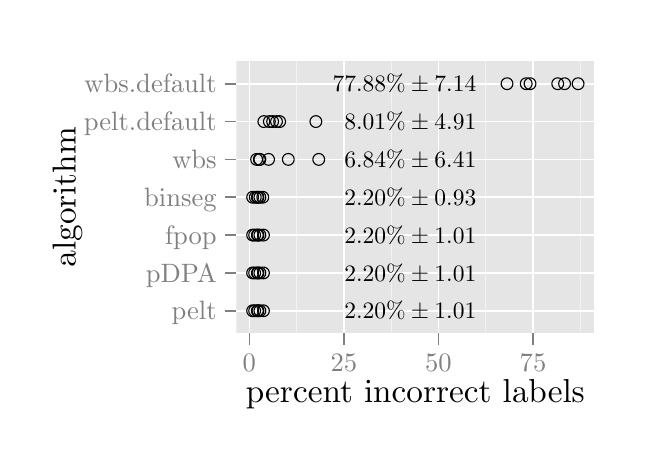
\begin{tikzpicture}[x=1pt,y=1pt]
\definecolor[named]{fillColor}{rgb}{1.00,1.00,1.00}
\path[use as bounding box,fill=fillColor,fill opacity=0.00] (0,0) rectangle (216.81,144.54);
\begin{scope}
\path[clip] (  0.00,  0.00) rectangle (216.81,144.54);
\definecolor[named]{drawColor}{rgb}{1.00,1.00,1.00}
\definecolor[named]{fillColor}{rgb}{1.00,1.00,1.00}

\path[draw=drawColor,line width= 0.6pt,line join=round,line cap=round,fill=fillColor] ( -0.00,  0.00) rectangle (216.81,144.54);
\end{scope}
\begin{scope}
\path[clip] ( 75.41, 34.03) rectangle (204.76,132.50);
\definecolor[named]{fillColor}{rgb}{0.90,0.90,0.90}

\path[fill=fillColor] ( 75.41, 34.03) rectangle (204.76,132.50);
\definecolor[named]{drawColor}{rgb}{0.95,0.95,0.95}

\path[draw=drawColor,line width= 0.3pt,line join=round] ( 97.19, 34.03) --
	( 97.19,132.50);

\path[draw=drawColor,line width= 0.3pt,line join=round] (131.36, 34.03) --
	(131.36,132.50);

\path[draw=drawColor,line width= 0.3pt,line join=round] (165.53, 34.03) --
	(165.53,132.50);

\path[draw=drawColor,line width= 0.3pt,line join=round] (199.70, 34.03) --
	(199.70,132.50);
\definecolor[named]{drawColor}{rgb}{1.00,1.00,1.00}

\path[draw=drawColor,line width= 0.6pt,line join=round] ( 75.41, 42.24) --
	(204.76, 42.24);

\path[draw=drawColor,line width= 0.6pt,line join=round] ( 75.41, 55.91) --
	(204.76, 55.91);

\path[draw=drawColor,line width= 0.6pt,line join=round] ( 75.41, 69.59) --
	(204.76, 69.59);

\path[draw=drawColor,line width= 0.6pt,line join=round] ( 75.41, 83.26) --
	(204.76, 83.26);

\path[draw=drawColor,line width= 0.6pt,line join=round] ( 75.41, 96.94) --
	(204.76, 96.94);

\path[draw=drawColor,line width= 0.6pt,line join=round] ( 75.41,110.61) --
	(204.76,110.61);

\path[draw=drawColor,line width= 0.6pt,line join=round] ( 75.41,124.29) --
	(204.76,124.29);

\path[draw=drawColor,line width= 0.6pt,line join=round] ( 80.10, 34.03) --
	( 80.10,132.50);

\path[draw=drawColor,line width= 0.6pt,line join=round] (114.27, 34.03) --
	(114.27,132.50);

\path[draw=drawColor,line width= 0.6pt,line join=round] (148.44, 34.03) --
	(148.44,132.50);

\path[draw=drawColor,line width= 0.6pt,line join=round] (182.61, 34.03) --
	(182.61,132.50);
\definecolor[named]{drawColor}{rgb}{0.00,0.00,0.00}

\node[text=drawColor,anchor=base east,inner sep=0pt, outer sep=0pt, scale=  0.85] at (162.11, 39.31) {$2.20\% \pm 1.01$};

\node[text=drawColor,anchor=base east,inner sep=0pt, outer sep=0pt, scale=  0.85] at (162.11, 52.99) {$2.20\% \pm 1.01$};

\node[text=drawColor,anchor=base east,inner sep=0pt, outer sep=0pt, scale=  0.85] at (162.11, 66.66) {$2.20\% \pm 1.01$};

\node[text=drawColor,anchor=base east,inner sep=0pt, outer sep=0pt, scale=  0.85] at (162.11, 80.34) {$2.20\% \pm 0.93$};

\node[text=drawColor,anchor=base east,inner sep=0pt, outer sep=0pt, scale=  0.85] at (162.11, 94.01) {$6.84\% \pm 6.41$};

\node[text=drawColor,anchor=base east,inner sep=0pt, outer sep=0pt, scale=  0.85] at (162.11,107.69) {$8.01\% \pm 4.91$};

\node[text=drawColor,anchor=base east,inner sep=0pt, outer sep=0pt, scale=  0.85] at (162.11,121.36) {$77.88\% \pm 7.14$};

\path[draw=drawColor,line width= 0.4pt,line join=round,line cap=round] ( 82.99, 42.24) circle (  2.13);

\path[draw=drawColor,line width= 0.4pt,line join=round,line cap=round] ( 83.91, 42.24) circle (  2.13);

\path[draw=drawColor,line width= 0.4pt,line join=round,line cap=round] ( 81.29, 42.24) circle (  2.13);

\path[draw=drawColor,line width= 0.4pt,line join=round,line cap=round] ( 83.22, 42.24) circle (  2.13);

\path[draw=drawColor,line width= 0.4pt,line join=round,line cap=round] ( 82.02, 42.24) circle (  2.13);

\path[draw=drawColor,line width= 0.4pt,line join=round,line cap=round] ( 85.20, 42.24) circle (  2.13);

\path[draw=drawColor,line width= 0.4pt,line join=round,line cap=round] ( 82.99, 55.91) circle (  2.13);

\path[draw=drawColor,line width= 0.4pt,line join=round,line cap=round] ( 83.91, 55.91) circle (  2.13);

\path[draw=drawColor,line width= 0.4pt,line join=round,line cap=round] ( 81.29, 55.91) circle (  2.13);

\path[draw=drawColor,line width= 0.4pt,line join=round,line cap=round] ( 83.22, 55.91) circle (  2.13);

\path[draw=drawColor,line width= 0.4pt,line join=round,line cap=round] ( 82.02, 55.91) circle (  2.13);

\path[draw=drawColor,line width= 0.4pt,line join=round,line cap=round] ( 85.20, 55.91) circle (  2.13);

\path[draw=drawColor,line width= 0.4pt,line join=round,line cap=round] ( 82.99, 69.59) circle (  2.13);

\path[draw=drawColor,line width= 0.4pt,line join=round,line cap=round] ( 83.91, 69.59) circle (  2.13);

\path[draw=drawColor,line width= 0.4pt,line join=round,line cap=round] ( 81.29, 69.59) circle (  2.13);

\path[draw=drawColor,line width= 0.4pt,line join=round,line cap=round] ( 83.22, 69.59) circle (  2.13);

\path[draw=drawColor,line width= 0.4pt,line join=round,line cap=round] ( 82.02, 69.59) circle (  2.13);

\path[draw=drawColor,line width= 0.4pt,line join=round,line cap=round] ( 85.20, 69.59) circle (  2.13);

\path[draw=drawColor,line width= 0.4pt,line join=round,line cap=round] ( 82.99, 83.26) circle (  2.13);

\path[draw=drawColor,line width= 0.4pt,line join=round,line cap=round] ( 83.91, 83.26) circle (  2.13);

\path[draw=drawColor,line width= 0.4pt,line join=round,line cap=round] ( 81.29, 83.26) circle (  2.13);

\path[draw=drawColor,line width= 0.4pt,line join=round,line cap=round] ( 83.22, 83.26) circle (  2.13);

\path[draw=drawColor,line width= 0.4pt,line join=round,line cap=round] ( 82.25, 83.26) circle (  2.13);

\path[draw=drawColor,line width= 0.4pt,line join=round,line cap=round] ( 84.96, 83.26) circle (  2.13);

\path[draw=drawColor,line width= 0.4pt,line join=round,line cap=round] (105.17, 96.94) circle (  2.13);

\path[draw=drawColor,line width= 0.4pt,line join=round,line cap=round] ( 83.91, 96.94) circle (  2.13);

\path[draw=drawColor,line width= 0.4pt,line join=round,line cap=round] ( 82.72, 96.94) circle (  2.13);

\path[draw=drawColor,line width= 0.4pt,line join=round,line cap=round] ( 83.70, 96.94) circle (  2.13);

\path[draw=drawColor,line width= 0.4pt,line join=round,line cap=round] ( 87.04, 96.94) circle (  2.13);

\path[draw=drawColor,line width= 0.4pt,line join=round,line cap=round] ( 94.18, 96.94) circle (  2.13);

\path[draw=drawColor,line width= 0.4pt,line join=round,line cap=round] ( 87.33,110.61) circle (  2.13);

\path[draw=drawColor,line width= 0.4pt,line join=round,line cap=round] ( 91.05,110.61) circle (  2.13);

\path[draw=drawColor,line width= 0.4pt,line join=round,line cap=round] ( 85.34,110.61) circle (  2.13);

\path[draw=drawColor,line width= 0.4pt,line join=round,line cap=round] ( 88.51,110.61) circle (  2.13);

\path[draw=drawColor,line width= 0.4pt,line join=round,line cap=round] ( 89.91,110.61) circle (  2.13);

\path[draw=drawColor,line width= 0.4pt,line join=round,line cap=round] (104.13,110.61) circle (  2.13);

\path[draw=drawColor,line width= 0.4pt,line join=round,line cap=round] (191.53,124.29) circle (  2.13);

\path[draw=drawColor,line width= 0.4pt,line join=round,line cap=round] (180.15,124.29) circle (  2.13);

\path[draw=drawColor,line width= 0.4pt,line join=round,line cap=round] (198.89,124.29) circle (  2.13);

\path[draw=drawColor,line width= 0.4pt,line join=round,line cap=round] (194.00,124.29) circle (  2.13);

\path[draw=drawColor,line width= 0.4pt,line join=round,line cap=round] (181.53,124.29) circle (  2.13);

\path[draw=drawColor,line width= 0.4pt,line join=round,line cap=round] (173.21,124.29) circle (  2.13);
\end{scope}
\begin{scope}
\path[clip] (  0.00,  0.00) rectangle (216.81,144.54);
\definecolor[named]{drawColor}{rgb}{0.50,0.50,0.50}

\node[text=drawColor,anchor=base east,inner sep=0pt, outer sep=0pt, scale=  0.96] at ( 68.30, 38.93) {pelt};

\node[text=drawColor,anchor=base east,inner sep=0pt, outer sep=0pt, scale=  0.96] at ( 68.30, 52.61) {pDPA};

\node[text=drawColor,anchor=base east,inner sep=0pt, outer sep=0pt, scale=  0.96] at ( 68.30, 66.28) {fpop};

\node[text=drawColor,anchor=base east,inner sep=0pt, outer sep=0pt, scale=  0.96] at ( 68.30, 79.96) {binseg};

\node[text=drawColor,anchor=base east,inner sep=0pt, outer sep=0pt, scale=  0.96] at ( 68.30, 93.63) {wbs};

\node[text=drawColor,anchor=base east,inner sep=0pt, outer sep=0pt, scale=  0.96] at ( 68.30,107.31) {pelt.default};

\node[text=drawColor,anchor=base east,inner sep=0pt, outer sep=0pt, scale=  0.96] at ( 68.30,120.98) {wbs.default};
\end{scope}
\begin{scope}
\path[clip] (  0.00,  0.00) rectangle (216.81,144.54);
\definecolor[named]{drawColor}{rgb}{0.50,0.50,0.50}

\path[draw=drawColor,line width= 0.6pt,line join=round] ( 71.14, 42.24) --
	( 75.41, 42.24);

\path[draw=drawColor,line width= 0.6pt,line join=round] ( 71.14, 55.91) --
	( 75.41, 55.91);

\path[draw=drawColor,line width= 0.6pt,line join=round] ( 71.14, 69.59) --
	( 75.41, 69.59);

\path[draw=drawColor,line width= 0.6pt,line join=round] ( 71.14, 83.26) --
	( 75.41, 83.26);

\path[draw=drawColor,line width= 0.6pt,line join=round] ( 71.14, 96.94) --
	( 75.41, 96.94);

\path[draw=drawColor,line width= 0.6pt,line join=round] ( 71.14,110.61) --
	( 75.41,110.61);

\path[draw=drawColor,line width= 0.6pt,line join=round] ( 71.14,124.29) --
	( 75.41,124.29);
\end{scope}
\begin{scope}
\path[clip] (  0.00,  0.00) rectangle (216.81,144.54);
\definecolor[named]{drawColor}{rgb}{0.50,0.50,0.50}

\path[draw=drawColor,line width= 0.6pt,line join=round] ( 80.10, 29.77) --
	( 80.10, 34.03);

\path[draw=drawColor,line width= 0.6pt,line join=round] (114.27, 29.77) --
	(114.27, 34.03);

\path[draw=drawColor,line width= 0.6pt,line join=round] (148.44, 29.77) --
	(148.44, 34.03);

\path[draw=drawColor,line width= 0.6pt,line join=round] (182.61, 29.77) --
	(182.61, 34.03);
\end{scope}
\begin{scope}
\path[clip] (  0.00,  0.00) rectangle (216.81,144.54);
\definecolor[named]{drawColor}{rgb}{0.50,0.50,0.50}

\node[text=drawColor,anchor=base,inner sep=0pt, outer sep=0pt, scale=  0.96] at ( 80.10, 20.31) {0};

\node[text=drawColor,anchor=base,inner sep=0pt, outer sep=0pt, scale=  0.96] at (114.27, 20.31) {25};

\node[text=drawColor,anchor=base,inner sep=0pt, outer sep=0pt, scale=  0.96] at (148.44, 20.31) {50};

\node[text=drawColor,anchor=base,inner sep=0pt, outer sep=0pt, scale=  0.96] at (182.61, 20.31) {75};
\end{scope}
\begin{scope}
\path[clip] (  0.00,  0.00) rectangle (216.81,144.54);
\definecolor[named]{drawColor}{rgb}{0.00,0.00,0.00}

\node[text=drawColor,anchor=base,inner sep=0pt, outer sep=0pt, scale=  1.20] at (140.09,  9.03) {percent incorrect labels};
\end{scope}
\begin{scope}
\path[clip] (  0.00,  0.00) rectangle (216.81,144.54);
\definecolor[named]{drawColor}{rgb}{0.00,0.00,0.00}

\node[text=drawColor,rotate= 90.00,anchor=base,inner sep=0pt, outer sep=0pt, scale=  1.20] at ( 17.30, 83.26) {algorithm};
\end{scope}
\end{tikzpicture}

  }
  \caption{Test error in neuroblastoma data set (percent incorrect labels,
    mean and standard deviation over 6 test folds). Note that pelt=pDPA=fpop 
    since these three algorithms recover the exact same segmentation.
    The ``default'' algorithms ignore the labels in the training set; 
    other algorithms pick the best scalar penalty or threshold
    using the training labels.}
  \label{tab:neuroblastoma-test-error}
\end{table}

\citet{HOCKING-breakpoints} proposed to benchmark the breakpoint
detection accuracy of segmentation models by using annotated regions
defined by experts when they visually inspected scatterplots of the
data. The neuroblastoma data are a set of 575 copy number microarrays
of neuroblastoma tumors, and each chromosome is a separate
segmentation problem. The benchmark is to use a training set of $n$
annotated chromosomes to learn a segmentation model, and then quantify
the annotation error on a test set. Let $d_1, \dots, d_n$ be the
number of data points to segment on each chromosome in the training
data set, and let $\mathbf y_1\in\RR^{d_1}, \dots, \mathbf
y_n\in\RR^{d_n}$ be the vectors of noisy data for each chromosome in
the training set.

Both pelt and pDPA have been applied to this benchmark by first
defining $\beta = \lambda d_i$ for all $i\in\{1, \dots, n\}$, and then
choosing the constant $\lambda$ that maximizes agreement with the
annotated regions in the training set. Since fpop computes the same
segmentation as pelt, we expected the same error rate for
fpop on the neuroblastoma benchmark.

As shown on
\url{http://cbio.ensmp.fr/~thocking/neuroblastoma/accuracy.html}, fpop
(fpop) achieves 2.2\% test error, the same as pDPA (cghseg.k) and pelt
(pelt.n).

In conclusion, the proposed fpop algorithm recovers the same
segmentation as pelt, so has the same breakpoint detection
accuracy.



\bibliographystyle{abbrvnat}
\bibliography{refs}

\end{document}
